% ======================================================================
\subsection{Symmetry reduction}

% ----------------------------------------------------------------------
\begin{frame}%[shrink]%[allowframebreaks]
  \frametitle{Continuous symmetry reduction}
  
  A flow
  $ \dot{\ssp} = \vel(\ssp) \,,\ssp(x, t) \in \reals^n$
  with $u(t)=f^t(u_0)$
  is {\color{blue} equivariant} under a continuous symmetry group $\Group$ if
  \begin{equation}
    \label{eq:equivariant}
    g \vel(\ssp) =  \vel(g \ssp) \,,\quad
    g f^t(\ssp) =  f^t(g \ssp)
    \quad \text{for any} \quad  g \in \Group
  \end{equation}
  \begin{equation}
    \LieEl(\gSpace)=e^{\gSpace \,\cdot\, \Lg }
    \,,\qquad
    \gSpace \cdot \Lg  = \sum_{a=1}^s \gSpace_a \Lg_a
    \,,
    \label{eq:Lie}
  \end{equation}
  
  \pause
  
  \begin{columns}[c]

    \column{0.6\textwidth}
    {\centering \htr{Slice} :\par}
    \[
      \braket{\sspRed - \slicep}{\sliceTan{}} = \braket{\sspRed}{\sliceTan{}} = 0
    \]
    \[
      \sliceTan{} = \groupTan(\slicep) = \Lg \, \slicep
    \]
    \[
      \sspRed = \LieEl^{-1}(\gSpace) \, \ssp
      \,.
    \]

    \column{0.3\textwidth}
    
    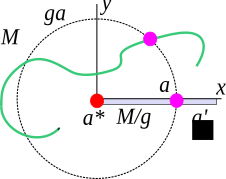
\includegraphics[width=1\linewidth]{FourierSlice}
    
  \end{columns}

\end{frame}

% ----------------------------------------------------------------------
\begin{frame}%[shrink]%[allowframebreaks]
  \frametitle{1st mode slice\footfullcite{BudCvi14}}
  \putssp

  \[
    R\,\ssp(x,t) = -\ssp(-x,t) \iff (b_k, c_k) \to (-b_k, c_k)
  \]
  \[
    \LieEl(\gSpace) \ssp(x, t) = \ssp (x+ \frac{\gSpace}{2\pi}L,t)
    \iff
    a_k \to e^{iq_k\gSpace} a_k
  \]
  
  \begin{columns}[c]
    \column{0.7\textwidth}

    \htr{1st mode slice} : 
    \[
      c_1 = 0 ,\, b_1 >0\,, \quad \text{that is,} \quad
      a_k \to e^{-iq_k\gSpace_1} a_k
    \]
    $\gSpace_1$ : the phase of $a_1$.

    \column{0.3\textwidth}
    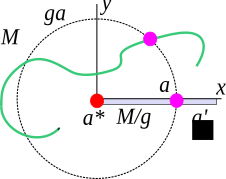
\includegraphics[width=1\linewidth]{FourierSlice}

  \end{columns}

\end{frame}

% ----------------------------------------------------------------------
\begin{frame}[shrink]%[allowframebreaks]
  \frametitle{\Reqva\ in the 1st mode slice}
  \putsym
 
  \htb{\reqv: 
    $\ssp(t) = \LieEl(t \, \velRel) \, \ssp(0)$
  }

  \begin{center} 
    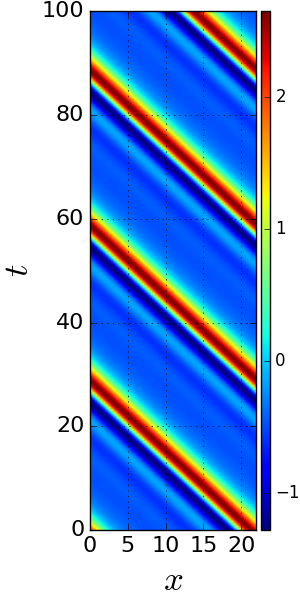
\includegraphics[width=0.2\textwidth]{ksReq1T100} 
    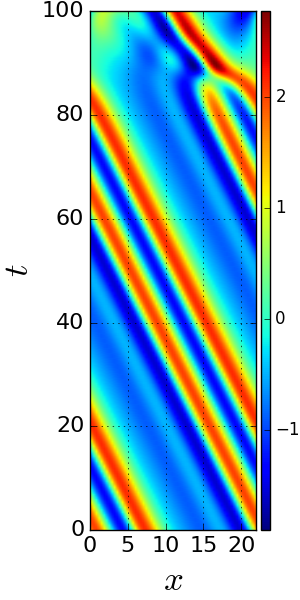
\includegraphics[width=0.2\textwidth]{ksReq2T100}
    $\implies$
    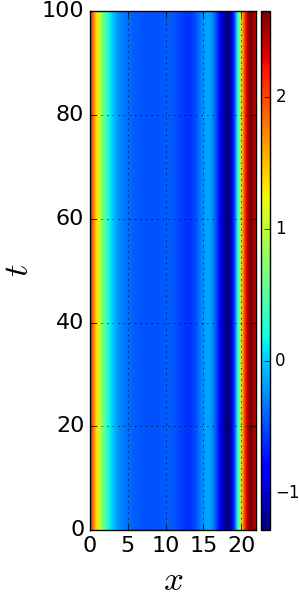
\includegraphics[width=0.2\textwidth]{ksReq1T100Red} 
    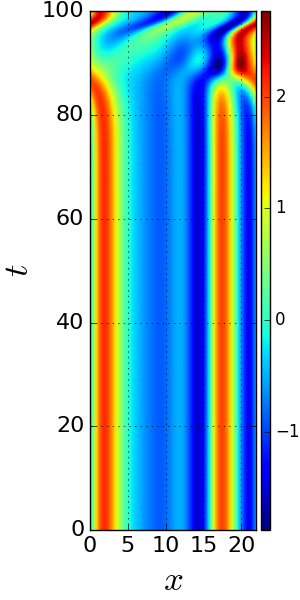
\includegraphics[width=0.2\textwidth]{ksReq2T100Red}
  \end{center}
  
\end{frame}

% ----------------------------------------------------------------------
\begin{frame}%[shrink]%[allowframebreaks]
  \frametitle{Pre\po s and \rpo s}
   
  \begin{center}
    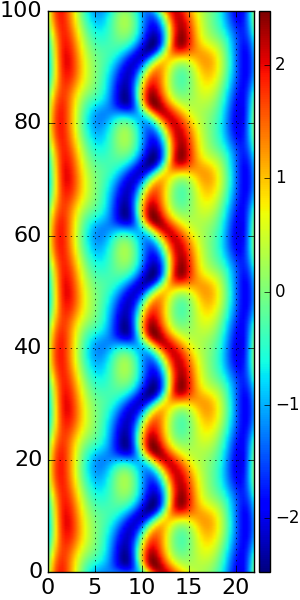
\includegraphics[width=0.16\textwidth]{ksppo1T100NoLabel}
    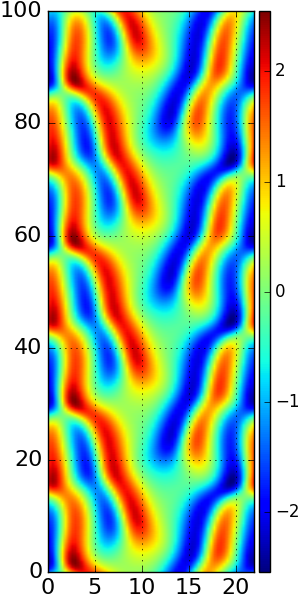
\includegraphics[width=0.16\textwidth]{ksppo2T100NoLabel}
    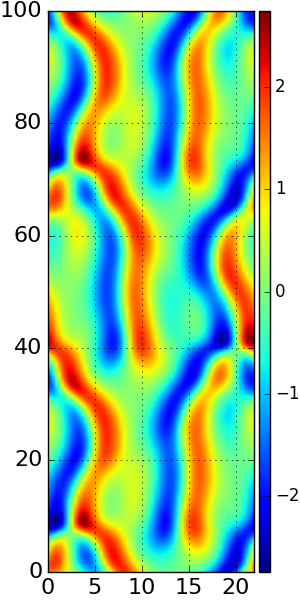
\includegraphics[width=0.16\textwidth]{ksppo3T100NoLabel}
    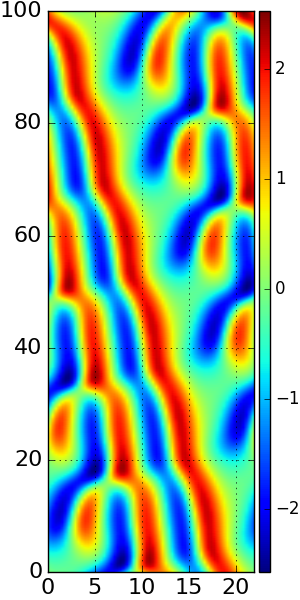
\includegraphics[width=0.16\textwidth]{ksrpo1T100NoLabel}
    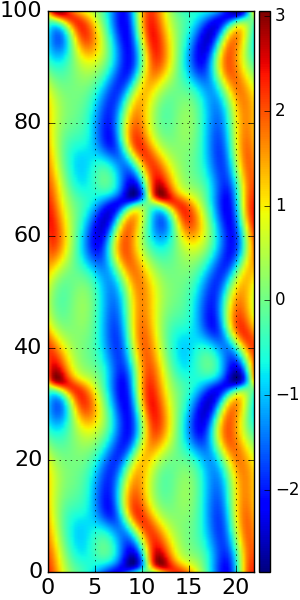
\includegraphics[width=0.16\textwidth]{ksrpo2T100NoLabel}
    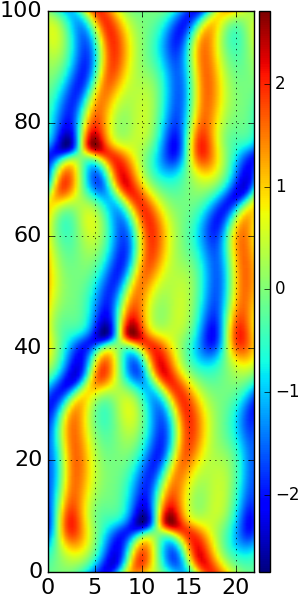
\includegraphics[width=0.16\textwidth]{ksrpo3T100NoLabel}

    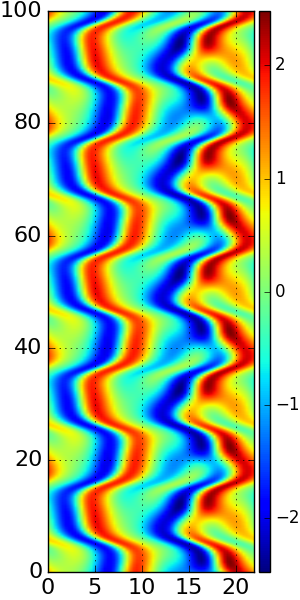
\includegraphics[width=0.16\textwidth]{ksppo1T100NoLabelRed}
    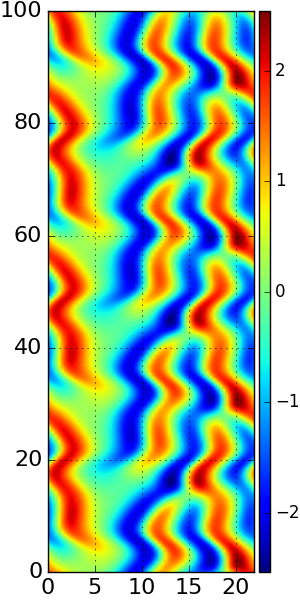
\includegraphics[width=0.16\textwidth]{ksppo2T100NoLabelRed}
    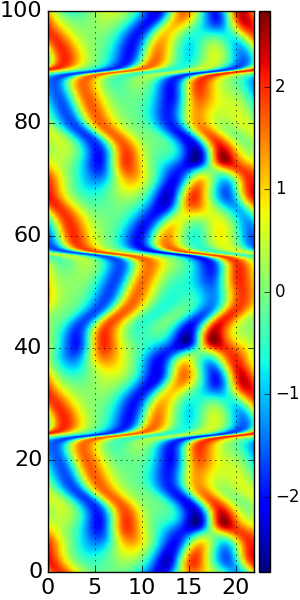
\includegraphics[width=0.16\textwidth]{ksppo3T100NoLabelRed}
    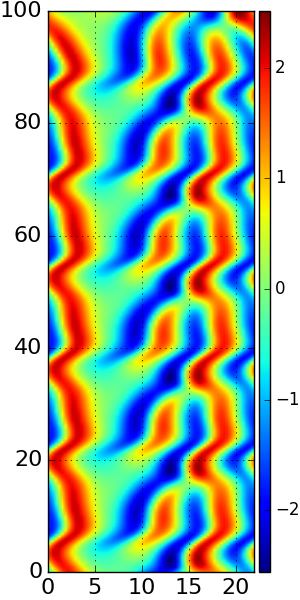
\includegraphics[width=0.16\textwidth]{ksrpo1T100NoLabelRed}
    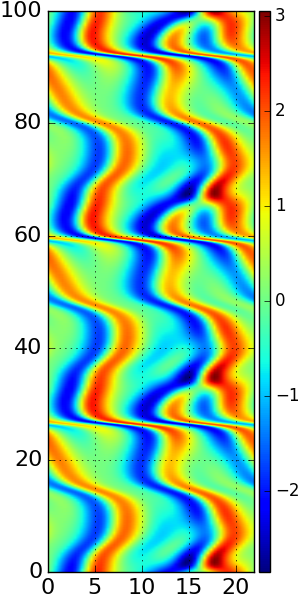
\includegraphics[width=0.16\textwidth]{ksrpo2T100NoLabelRed}
    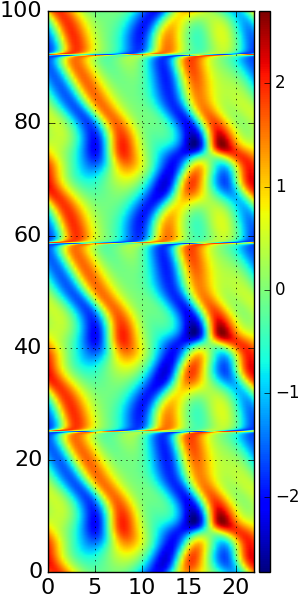
\includegraphics[width=0.16\textwidth]{ksrpo3T100NoLabelRed}
  \end{center}
  
\end{frame}
